% Talk slides (<= 15 min): research fashions at ICLR 2017-2026, with the held-out replication. Academic Beamer style.
% Build: python make_figures.py && pdflatex slides && pdflatex slides
\documentclass[aspectratio=169,11pt]{beamer}
\usetheme{Madrid}
\usefonttheme{professionalfonts}
\usepackage[T1]{fontenc}
\usepackage{lmodern}
\usepackage{amsmath}
\usepackage{booktabs}
\usepackage{tabularx}
\usepackage{tikz}
\usetikzlibrary{positioning,arrows.meta}

\definecolor{navy}{HTML}{1F3A68}
\definecolor{crimson}{HTML}{A31F34}
\definecolor{note}{HTML}{5A5A5A}
\usecolortheme[named=navy]{structure}
\setbeamercolor{alerted text}{fg=crimson}
\setbeamercolor{block title}{bg=navy!85,fg=white}
\setbeamercolor{block body}{bg=navy!6,fg=black}
\setbeamertemplate{blocks}[rounded][shadow=false]
\setbeamertemplate{navigation symbols}{}
\setbeamertemplate{caption}[numbered]
\setbeamerfont{caption}{size=\scriptsize}
\setbeamertemplate{itemize items}[circle]
\setbeamertemplate{enumerate items}[default]
\setbeamertemplate{section in toc}[sections numbered]

\newcommand{\pp}{\,pp}
\newcommand{\gnote}[1]{{\color{note}#1}}
\newcommand{\rc}[1]{{\color{note}\footnotesize(#1)}}

\title[Riding the Wave?]{Riding the Wave?}
\subtitle{Who Starts, Follows and Gains from ML Research Trends\texorpdfstring{\\[0.3em]
  \small A Pre-registered Study of ICLR Submissions, 2017--2026:\\ 43,480 Discovery and 11,099 Held-out Papers}{}}
\author[{[Your name]}]{[Your name]}
\institute[{[Institution]}]{[Department], [Institution]}
\date[{[Date]}]{[Venue / seminar] \quad [Date]}
\pdfstringdefDisableCommands{\def\translate#1{#1}}

\begin{document}

\begin{frame}
  \titlepage
\end{frame}

\begin{frame}{Outline}
  \tableofcontents
\end{frame}

% ============================================================================ 1
\section{Motivation and Research Questions}

\begin{frame}{Motivation: Research Fashions in Machine Learning}
  \begin{table}
    \centering
    \begin{tabular}{@{}lrr@{}}
      \toprule
      Share of ICLR submissions that \ldots & 2017 & 2026 \\
      \midrule
      propose a new architecture & 24\% & 8\% \\
      build on a foundation model & 0.3\% & 54\% \\
      carry a branded title (``NAME: subtitle'') & 9\% & 41\% \\
      \bottomrule
    \end{tabular}
    \caption{Field-wide shifts in content and in style.}
  \end{table}
  \begin{itemize}
    \item ML research moves in waves, in \emph{what} is studied and in \emph{how} it is presented.
    \item Are these \alert{fashions}? If so: what do they displace, who drives them, and are followers rewarded?
  \end{itemize}
\end{frame}

\begin{frame}{Research Questions and Pre-registered Hypotheses}
  \begin{table}
    \centering\small
    \begin{tabularx}{\textwidth}{@{}l >{\raggedright\arraybackslash}X c@{}}
      \toprule
      Question & Key hypothesis & Predicted sign \\
      \midrule
      \textbf{RQ1 Rise}: what does a fashion displace? &
        \textbf{H1d}: prior foundation-model (FM) adoption in a topic $\to$ share of new-architecture papers & $-$ \\
      \addlinespace
      \textbf{RQ2 Following}: who introduces new work? &
        \textbf{H2b}: newcomer paper $\to$ new-method paper & $-$ \\
      & \textbf{H2c}: newcomer paper $\to$ benchmark/evaluation paper & $+$ \\
      \addlinespace
      \textbf{RQ3 Reward}: are followers rewarded? &
        \textbf{H3a}: topic maturity (prior papers in topic) $\to$ acceptance & $-$ \\
      \bottomrule
    \end{tabularx}
    \caption{Selected hypotheses. Ten hypotheses registered in total.}
  \end{table}
  \gnote{\footnotesize Our RQ2 prediction followed the fashion view: newcomers imitate, insiders innovate.}
\end{frame}

\begin{frame}{Related Work and Positioning}
  \begin{columns}[T]
    \begin{column}{0.49\textwidth}
      \textbf{Two views of who drives new work}
      \begin{itemize}
        \item \emph{Fashion and herding}: ideas spread by imitation \rc{Abrahamson, 1991; Bikhchandani et al., 1992}
          $\Rightarrow$ newcomers follow
        \item \emph{Outsider innovation}: new entrants bring new ideas \rc{Azoulay et al., 2019};
          tradition vs.\ innovation \rc{Foster et al., 2015}
        \item Team size: large teams develop, small teams disrupt \rc{Wu et al., 2019}
      \end{itemize}
    \end{column}
    \begin{column}{0.49\textwidth}
      \textbf{Meta-research on ML}
      \begin{itemize}
        \item Benchmark concentration \rc{Koch et al., 2021}
        \item Values encoded in ML papers \rc{Birhane et al., 2022}
      \end{itemize}
      \vspace{0.3em}
      \textbf{Measurement challenges we address}
      \begin{enumerate}
        \item Survivorship: only published papers observed
        \item Hindsight: topics defined on the full period
        \item Forking paths \rc{Gelman \& Loken, 2014} $\Rightarrow$ pre-registration \rc{Nosek et al., 2018}
      \end{enumerate}
    \end{column}
  \end{columns}
\end{frame}

% ============================================================================ 2
\section{Data and Measurement}

\begin{frame}{Data and Measurement}
  \footnotesize
  \begin{table}
    \centering
    \begin{tabularx}{\textwidth}{@{}l X X@{}}
      \toprule
      Construct & Operationalisation & Validation \\
      \midrule
      Corpus & 43,480 discovery + 11,099 held-out ICLR submissions (released former confirmation split),
        2017--2026, from OpenReview: accepted, rejected, withdrawn &
        Held-out: never analysed before its single registered run; a pre-registered out-of-sample replication, not a
        certified untouched holdout \\
      Topic & SPECTER2 embeddings of title + abstract \rc{Singh et al., 2023}; $k = 100$ clusters; held-out papers
        placed on the frozen maps &
        Agreement with ICLR areas: NMI 0.30 (keyword baseline 0.27); robust to $k = 75, 150$ \\
      Contribution type & LLM with a fixed codebook: method, benchmark/evaluation, empirical, theory, other &
        Blind second pass: $\kappa = 0.93$ on both splits (held-out: 555 papers) \\
      Newcomer paper & No author has an earlier ICLR submission \emph{in the topic} (73\% of papers) &
        Exact OpenReview author IDs \\
      Acceptance & Final decision & Sealed in code until each split's single registered run (held-out: the earlier
        keyword grid's overlap is unknown) \\
      \bottomrule
    \end{tabularx}
    \caption{Constructs, measures and checks.}
  \end{table}
\end{frame}

% ============================================================================ 3
\section{Methodological Contribution: Hindsight Bias in Topic Maps}

\begin{frame}{Hindsight Bias in Topic Maps}
  \begin{columns}[c]
    \begin{column}{0.58\textwidth}
      \begin{figure}
        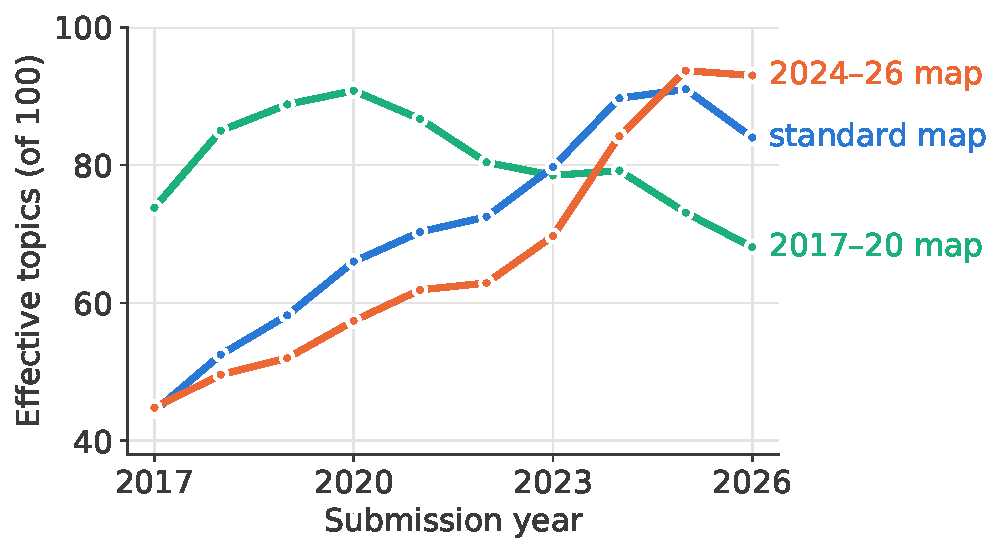
\includegraphics[width=\textwidth]{figs/hindsight_diversity.pdf}
        \caption{Effective number of topics per year under three $k = 100$ maps fitted on different years.}
      \end{figure}
    \end{column}
    \begin{column}{0.40\textwidth}
      \small
      \begin{itemize}
        \item 69\% of submissions are from 2024--26: a map fitted on all years is a map of the \emph{present}.
        \item Each map finds peak diversity in the years used to fit it.
      \end{itemize}
      \begin{block}{Implication}
        Topic maps are not neutral preprocessing: the fitting window shapes the history one observes.
      \end{block}
    \end{column}
  \end{columns}
\end{frame}

\begin{frame}{Consequence: Substantive Conclusions Depend on the Map}
  \small
  \begin{itemize}
    \item Emerging topics (${\geq}3\times$ growth): \textbf{8} with the 2017--20 map vs.\ \textbf{29} with the standard map.
    \item Small topics `predict' 2-year growth on the standard map ($R^2 = 0.28$), not on the 2017--20 map ($-0.03$).
      \gnote{(Post hoc.)}
    \item Do topics age, from new methods towards benchmarks? Same papers, same model:
  \end{itemize}
  \vspace{-0.6em}
  \begin{figure}
    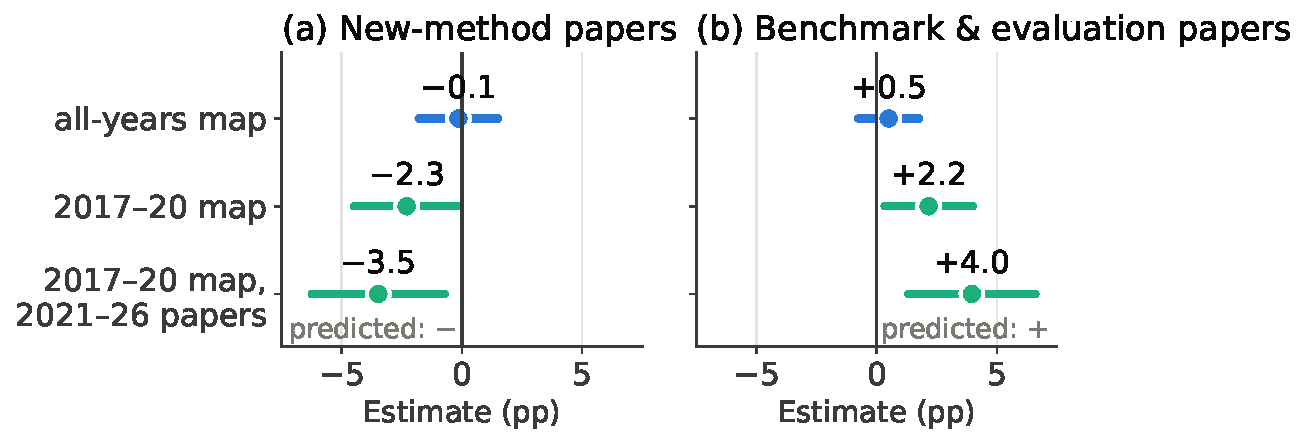
\includegraphics[width=0.60\textwidth]{figs/lifecycle_flip.pdf}
    \caption{Coefficient on topic maturity (log prior papers), 95\% CI. Early-map rows are exploratory.}
  \end{figure}
  \vspace{-0.7em}
  \centering\gnote{$\Rightarrow$ Every registered result must also pass two hindsight checks (early-year and
  year-balanced maps).}
\end{frame}

% ============================================================================ 4
\section{Empirical Strategy}

\begin{frame}{Empirical Strategy}
  \begin{columns}[T]
    \begin{column}{0.52\textwidth}
      \textbf{Specification} (linear probability model)
      \[
        y_i \;=\; \beta\, x_i \;+\; \mu_{k(i)} \;+\; \tau_{t(i)} \;+\; \varepsilon_i
      \]
      \vspace{-1.2em}
      \footnotesize
      \begin{itemize}
        \item $y_i \in \{0,1\}$: paper type or acceptance; $x_i$: e.g.\ newcomer paper
        \item $\mu_k$, $\tau_t$: topic and year fixed effects (topic $\times$ year for RQ2)
        \item Standard errors clustered by topic (100 clusters)
      \end{itemize}
      \small\textbf{Decision rule} (registered). Supported only if:
      \footnotesize
      \begin{enumerate}
        \item predicted sign, and Holm-adjusted $p < 0.05$;
        \item same sign in ${\geq}75\%$ of 9--11 alternative specifications;
        \item same sign under both hindsight checks.
      \end{enumerate}
    \end{column}
    \begin{column}{0.45\textwidth}
      \begin{block}{Protocol}
        \footnotesize
        Pre-registered; variables built blind to acceptance; 12,400 simulation runs; code and inputs frozen
        (SHA-256); a single run; every estimate reported.
      \end{block}
      \vspace{-0.3em}
      \begin{block}{Simulation finding}
        \footnotesize No-effect data: clustered SEs rejected up to \alert{12.6\%} at nominal 5\%, so RQ2 gets two
        extra checks (two-way clustering, a stress test).
      \end{block}
      \vspace{-0.3em}
      \begin{block}{Held-out rule (registered)}
        \footnotesize Registered tests only; one-sided $\alpha = 0.05$; frozen code and topic maps; features built on
        discovery + held-out papers.
      \end{block}
    \end{column}
  \end{columns}
\end{frame}

% ============================================================================ 5
\section{Results}

\begin{frame}{RQ1: Foundation-Model Adoption and New Architectures}
  \begin{columns}[c]
    \begin{column}{0.44\textwidth}
      \begin{figure}
        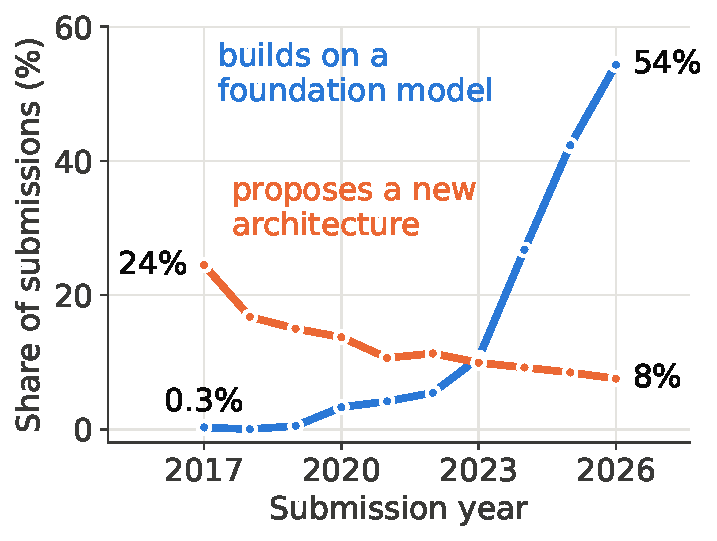
\includegraphics[width=\textwidth]{figs/fm_trend.pdf}
        \caption{Field-wide trends (descriptive).}
      \end{figure}
    \end{column}
    \begin{column}{0.54\textwidth}
      \small
      Within topic, net of year effects: prior FM adoption vs.\ new-architecture papers.
      \begin{table}
        \centering\footnotesize\setlength{\tabcolsep}{4pt}
        \begin{tabular}{@{}lrr@{}}
          \toprule
          & Discovery & Held-out \\
          \midrule
          $\hat\beta$ (0 $\to$ 100\% FM) & $-0.080$ & $\mathbf{-0.110}$ \\
          (SE) & (0.021) & (0.036) \\
          95\% CI & [$-0.121$, $-0.038$] & [$-0.181$, $-0.039$] \\
          $p$ & Holm 0.001 & one-sided 0.001 \\
          Same sign (specs) & 9 / 9 & 9 / 9 \\
          $N$ & 42,990 & 10,978 \\
          \bottomrule
        \end{tabular}
      \end{table}
      \vspace{-0.5em}
      \begin{itemize}
        \item H1d \textbf{supported}, and \textbf{replicated} on the held-out papers.
        \item Topics at 50\% vs.\ 10\% FM adoption: about \alert{one third fewer} new-architecture papers
          (discovery; base 9\%).
      \end{itemize}
    \end{column}
  \end{columns}
\end{frame}

\begin{frame}{RQ2: Newcomers and Contribution Types}
  \begin{columns}[c]
    \begin{column}{0.50\textwidth}
      \begin{figure}
        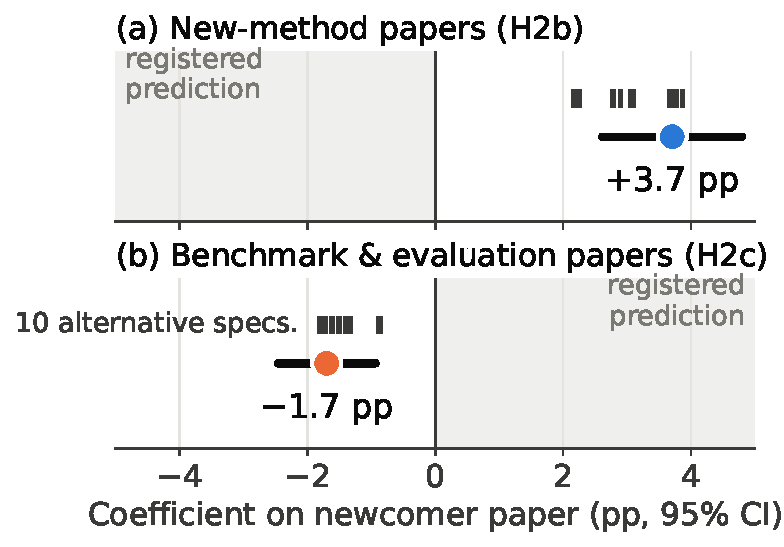
\includegraphics[width=\textwidth]{figs/newcomers.pdf}
        \caption{Discovery; topic $\times$ year FE; grey: predicted side.}
      \end{figure}
    \end{column}
    \begin{column}{0.48\textwidth}
      \footnotesize
      \begin{table}
        \centering\footnotesize\setlength{\tabcolsep}{3pt}
        \begin{tabular}{@{}lrr@{}}
          \toprule
          & H2b (method) & H2c (bench.) \\
          \midrule
          Discovery $\hat\beta$ (SE) & $+0.037$ (0.006) & $-0.017$ (0.004) \\
          Same sign & 10/10 & 10/10 \\
          Held-out $\hat\beta$ & $\mathbf{+0.036}$ & $\mathbf{-0.021}$ \\
          95\% CI & [$0.015$, $0.057$] & [$-0.033$, $-0.008$] \\
          Base rate: disc. & 75\% & 7.7\% \\
          \quad held-out & 75\% & 7.9\% \\
          \bottomrule
        \end{tabular}
      \end{table}
      \vspace{-0.8em}
      \begin{itemize}
        \item Discovery: both \alert{opposite} to prediction (wild cluster bootstrap $p < 0.001$; $N = 42{,}315$)
        \item Held-out: reversed predictions H2b$'$/H2c$'$ (registered) \textbf{supported} (one-sided Holm
          $p = 0.001$ each; $N = 10{,}718$)
        \item Consistent with outsider innovation, not with herding
      \end{itemize}
      \gnote{\scriptsize Most of the H2c gap goes with team size; H2b does not.}
    \end{column}
  \end{columns}
\end{frame}

\begin{frame}{RQ3: Is Following the Fashion Rewarded?}
  \begin{table}
    \centering\footnotesize
    \begin{tabularx}{\textwidth}{@{}X r r l@{}}
      \toprule
      Association with acceptance & Discovery & Held-out & Status \\
      \midrule
      Topic maturity, per log unit of prior papers (H3a) & $-1.7$\pp{} (SE 1.0) & $-1.5$\pp{} (SE 1.9)
        & inconclusive in both \\
      Branded title & ratio 1.02 & not tested & exploratory \\
      New arch.\ $\times$ prior FM adoption (0 $\to$ 100\%) & $+8.3$\pp{} (SE 3.5) & not tested
        & exploratory, $p = 0.02$ \\
      \bottomrule
    \end{tabularx}
    \caption{Topic and year fixed effects; SEs clustered by topic; decided papers, 2018--2026 (H3a: $N = 32{,}190$,
    MDE$_{80}$ 4\pp; held-out $N = 8{,}185$, MDE$_{80}$ 4.8\pp, one-sided $p = 0.21$).}
  \end{table}
  \begin{block}{Reading}
    \small No detectable reward for following the fashion at review; the crowding test is inconclusive in both
    splits. If anything, papers that go against the tide (architectures where FMs dominate) do relatively better
    (exploratory).
  \end{block}
\end{frame}

\begin{frame}{Far Jumps Go with Lower Acceptance (Post Hoc, Replicated)}
  \begin{columns}[c]
    \begin{column}{0.53\textwidth}
      \begin{figure}
        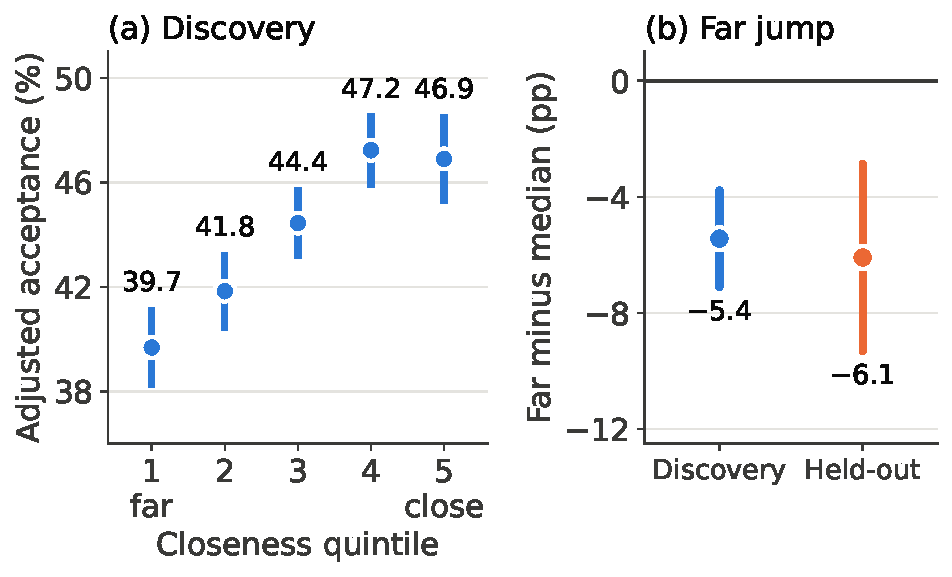
\includegraphics[width=0.92\textwidth]{figs/far_jump.pdf}
        \caption{Decided papers with ${\geq}1$ experienced author, 2023--26 (E1 sample: discovery 20,430; held-out
        5,344). Closeness: highest cosine between the abstract and an experienced co-author's earlier ICLR work.
        (b) 10th percentile minus median. 95\% CIs.}
      \end{figure}
    \end{column}
    \begin{column}{0.45\textwidth}
      \footnotesize
      \begin{itemize}
        \item Far jump from the team's own record vs.\ median: $-5.4$\pp{} in discovery; \alert{$-6.1$\pp{}}
          held-out (CI $-9.3$ to $-2.9$; Holm $p = 0.005$)
        \item Same author, closer paper: $+0.55$\pp{} (discovery), $+1.06$\pp{} (held-out) per $+0.1$ cosine
        \item Near vs.\ median: not lower ($+1.7$\pp{} discovery; $+2.3$\pp{} held-out, not registered)
        \item \textbf{Not replicated}: the field-novelty floor. Least-novel fifth: $-3.3$\pp{} in discovery,
          $-0.1$\pp{} held-out (CI $-3.5$ to $+3.2$); uninformative by the registered rule (power 0.47,
          MDE$_{80}$ 5.4\pp)
      \end{itemize}
      \gnote{\scriptsize Post hoc in discovery; held-out tests registered before the run. Held-out: post-decision
      abstracts, no cleaned-text check. Associations: co-author choice and failed projects not controlled.}
    \end{column}
  \end{columns}
\end{frame}

\begin{frame}{Why Do Some Areas Lose Favour? (Post Hoc)}
  \begin{columns}[c]
    \begin{column}{0.45\textwidth}
      \begin{figure}
        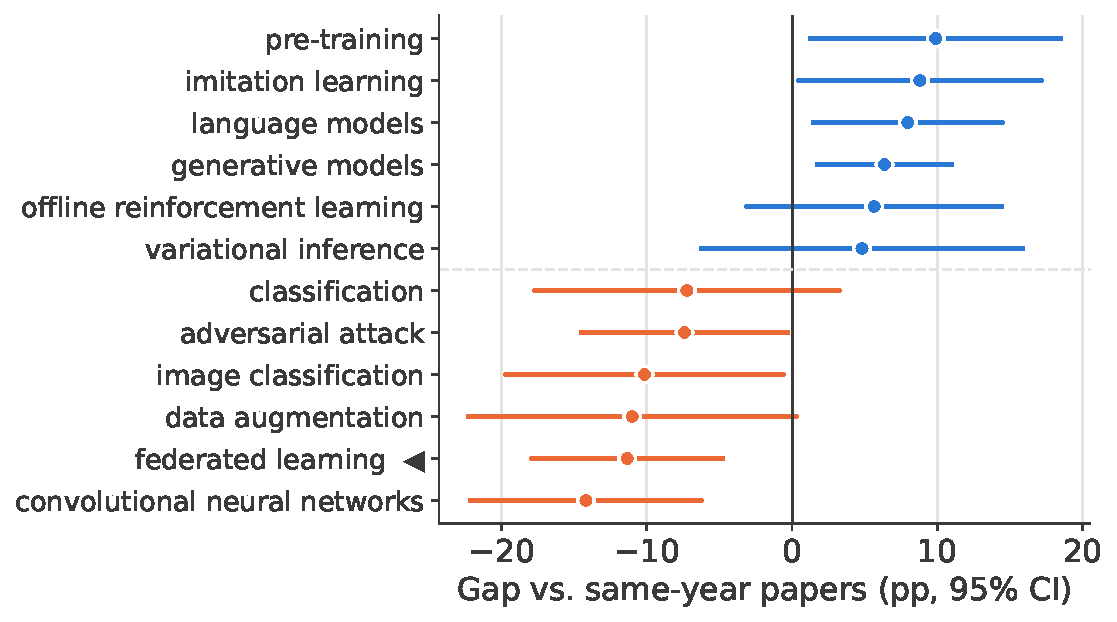
\includegraphics[width=\textwidth]{figs/area_ranking.pdf}
        \caption{Acceptance gap vs.\ same-year papers, 2018--2026: six highest and six lowest author keywords
        (${\geq}5$ years of data; 32,190 decided papers).}
      \end{figure}
    \end{column}
    \begin{column}{0.53\textwidth}
      \scriptsize
      \textbf{Pattern} ($\pm$10\pp): current-wave and specialist areas above; older or entry-level areas below.
      \par\smallskip
      \textbf{Candidate explanations (checked across 50 keywords):}
      \begin{itemize}\setlength{\itemsep}{1pt}
        \item \emph{Entry points attract newcomers:} 85--88\% of CNN and classification papers come from authors new
          to the topic; more newcomers, lower acceptance ($\rho = -0.40$, $p = 0.004$).
        \item \emph{Paradigm moved on:} CNN and image-classification shares peaked in 2018 (2026: 5\% and 24\% of
          peak); incremental gains on saturated benchmarks may face a higher bar (untested).
        \item \emph{Cooling area:} federated learning, with established authors and a falling share since 2023.
        \item \emph{Not} paper type, team size (adjusted vs.\ raw gaps $r = 0.97$) \emph{or} the FM wave (FM share
          vs.\ acceptance $\rho = 0.07$).
      \end{itemize}
      \gnote{\tiny Associations, not causes; no area survives correction for 68 tests. Held-out: edges shrink
      ($0.60\times$) but persist; FL gap not confirmed.}
    \end{column}
  \end{columns}
\end{frame}

% ============================================================================ 6
\section{Held-out Replication}

\begin{frame}[t]{Do the Results Hold on Held-out Papers?}
  \vspace{-0.4em}
  \begin{table}
    \centering\scriptsize\setlength{\tabcolsep}{4.5pt}\renewcommand{\arraystretch}{0.92}
    \setlength{\abovecaptionskip}{3pt}
    % generated by make_figures.replication_table(); do not edit by hand
\begin{tabular}{@{}l c r l r l@{}}
\toprule
Test & Pred. & Discovery & Held-out [95\% CI] & One-sided $p$ & Verdict \\
\midrule
\multicolumn{6}{@{}l}{\emph{Registered hypotheses (one-sided $p$, Holm-adjusted within family)}} \\
\textbf{H1d} FM adoption (0 $\to$ 1) $\to$ new arch. & $-$ & $-$8.0 & $-$11.0 [$-$18.1, $-$3.9] & 0.001 & supported \\
\textbf{H2b$'$} newcomer $\to$ method paper & $+$ & $+$3.7 & $+$3.6 [$+$1.5, $+$5.7] & 0.001 & supported \\
\textbf{H2c$'$} newcomer $\to$ benchmark paper & $-$ & $-$1.7 & $-$2.1 [$-$3.3, $-$0.8] & 0.001 & supported \\
\textbf{H3a} maturity (log) $\to$ acceptance & $-$ & $-$1.7 & $-$1.5 [$-$5.2, $+$2.2] & 0.21 & inconclusive\textsuperscript{\dag} \\
\textbf{H4-FL} FL keyword $\to$ acceptance & $-$ & $-$11.3 & $-$4.9 [$-$15.4, $+$5.7] & 0.14 & not supported\textsuperscript{\dag} \\
\addlinespace[2pt]
\multicolumn{6}{@{}l}{\emph{PH5 primary (post hoc in discovery; one-sided $p$, Holm-adjusted over the pair)}} \\
\textbf{E1} far jump (p10 $-$ median) & $-$ & $-$5.4 & $-$6.1 [$-$9.3, $-$2.9] & 0.005 & supported \\
\textbf{P1b} least-novel $-$ middle fifth & $-$ & $-$3.3 & $-$0.1 [$-$3.5, $+$3.2] & 0.47 & not supported\textsuperscript{\dag} \\
\addlinespace[2pt]
\multicolumn{6}{@{}l}{\emph{PH5 secondary (one-sided $p$, unadjusted)}} \\
\textbf{E4} within author, per $+$0.1 cos & $+$ & $+$0.55 & $+$1.06 [$+$0.23, $+$1.89] & 0.006 & supported \\
\textbf{Teams H1} one insider vs none & $+$ & $+$3.4 & $+$3.9 [$+$0.3, $+$7.5] & 0.017 & supported \\
\textbf{A1} Emerging $-$ Mainstream keyword & $+$ & $+$2.7 & $+$3.3 [$-$0.2, $+$6.7] & 0.031 & supported \\
\textbf{Premia $b$} topic edges (early map) & $0<b<1$ & 0.38\textsuperscript{\ddag} & 0.60 [0.32, 0.88] & 0.003 & supported \\
\bottomrule
\end{tabular}

    \caption{11,099 released former confirmation papers this study had never analysed: a pre-registered out-of-sample
    replication, not a certified untouched holdout. Supported: one-sided $p < 0.05$, Holm within families (so a 95\% CI
    can cross 0). pp unless noted. \dag\,Below MDE$_{80}$: uninformative. \ddag\,Within-discovery slope.
    Also registered: H4-FL trend, P7 not supported; premia EB supported.}
  \end{table}
\end{frame}

% ============================================================================ 7
\section{Conclusion}

\begin{frame}{Contributions}
  \begin{enumerate}
    \item \textbf{Methodological.} Topic maps fitted with hindsight manufacture emerging topics and can reverse trend
      conclusions; early-year maps provide a cheap check.
    \item \textbf{Design.} A pre-registered, outcome-blind, simulation-checked, single-run protocol for
      science-of-science studies, with a registered held-out replication.
    \item \textbf{Substantive} (associations).
      \small
      \begin{itemize}
        \item \textbf{Replicated:} where foundation models spread, new architectures fade (H1d); newcomer papers lean
          towards new methods and away from benchmarks (H2b$'$/H2c$'$); far jumps from the team's own record go with
          lower acceptance (post hoc in discovery).
        \item \textbf{Not replicated:} the field-novelty floor (least-novel fifth); the held-out test was
          uninformative (power 0.47, MDE$_{80}$ 5.4\pp).
        \item \textbf{Not confirmed:} the federated-learning acceptance gap; the held-out test was uninformative
          (134 papers, MDE$_{80}$ 14.5\pp).
        \item \textbf{Inconclusive} in both splits: crowded (mature) topics and acceptance.
      \end{itemize}
  \end{enumerate}
\end{frame}

\begin{frame}{Limitations and Future Work}
  \begin{columns}[T]
    \begin{column}{0.50\textwidth}
      \textbf{Limitations}
      \small
      \begin{itemize}
        \item One venue (ICLR)
        \item Associations, not causal effects
        \item LLM labels: consistent ($\kappa = 0.93$), not yet human-validated
        \item Camera-ready text: the discovery cleaned-text checks held; no such check for held-out papers
        \item Held-out papers are a released former holdout, not certified untouched
        \item Pooled re-run (54,579 papers) is exploratory and confirms nothing
        \item 2021 author-ID change undercounts incumbents (expected bias towards zero)
      \end{itemize}
    \end{column}
    \begin{column}{0.46\textwidth}
      \textbf{Future work}
      \small
      \begin{itemize}
        \item A prospective test on future ICLR submissions
        \item Extension to ACL Anthology / ARR
        \item Human validation of contribution labels
        \item Review scores: reviewers vs.\ final decisions
      \end{itemize}
    \end{column}
  \end{columns}
\end{frame}

\begin{frame}
  \centering
  \vspace{2em}
  {\Large Thank you}\\[1em]
  Questions and comments welcome\\[0.5em]
  \gnote{\small [email]}
\end{frame}

\begin{frame}{References}
  \scriptsize
  \begin{itemize}\setlength{\itemsep}{1pt}
    \item[] Abrahamson, E. (1991). Managerial fads and fashions: The diffusion and rejection of innovations.
      \emph{Academy of Management Review}, 16(3), 586--612.
    \item[] Azoulay, P., Fons-Rosen, C., \& Graff Zivin, J. S. (2019). Does science advance one funeral at a time?
      \emph{American Economic Review}, 109(8), 2889--2920.
    \item[] Bikhchandani, S., Hirshleifer, D., \& Welch, I. (1992). A theory of fads, fashion, custom, and cultural
      change as informational cascades. \emph{Journal of Political Economy}, 100(5), 992--1026.
    \item[] Birhane, A., Kalluri, P., Card, D., Agnew, W., Dotan, R., \& Bao, M. (2022). The values encoded in machine
      learning research. In \emph{Proceedings of ACM FAccT}.
    \item[] Cameron, A. C., Gelbach, J. B., \& Miller, D. L. (2008). Bootstrap-based improvements for inference with
      clustered errors. \emph{Review of Economics and Statistics}, 90(3), 414--427.
    \item[] Foster, J. G., Rzhetsky, A., \& Evans, J. A. (2015). Tradition and innovation in scientists' research
      strategies. \emph{American Sociological Review}, 80(5), 875--908.
    \item[] Gelman, A., \& Loken, E. (2014). The statistical crisis in science. \emph{American Scientist}, 102(6),
      460--465.
    \item[] Koch, B., Denton, E., Hanna, A., \& Foster, J. G. (2021). Reduced, reused and recycled: The life of a
      dataset in machine learning research. In \emph{NeurIPS Datasets and Benchmarks Track}.
    \item[] Nosek, B. A., Ebersole, C. R., DeHaven, A. C., \& Mellor, D. T. (2018). The preregistration revolution.
      \emph{Proceedings of the National Academy of Sciences}, 115(11), 2600--2606.
    \item[] Singh, A., D'Arcy, M., Cohan, A., Downey, D., \& Feldman, S. (2023). SciRepEval: A multi-format benchmark
      for scientific document representations. In \emph{Proceedings of EMNLP}.
    \item[] Wu, L., Wang, D., \& Evans, J. A. (2019). Large teams develop and small teams disrupt science and
      technology. \emph{Nature}, 566(7744), 378--382.
  \end{itemize}
\end{frame}

\end{document}
